\chapter{System Development}

For the purposes of this work, the tasks that users are asked to complete are moving the swarm in space, patrolling areas, moving objects, and directing the swarm to form various formations. 

\section{Compilation of robot programs}

The user interface may be able to drive the re-imagining of the robots as a unified swarm, and so alter the user's interaction with the swarm, by depicting the group in different ways \citep{manning2015heuristic}.
The base case is to simply display all the units as individuals, but this may not be useful for the operator \citep{coppin2012controlling}. 
Other approaches include an amorphous shape covering the area occupied by the swarm, an amorphous shape with density shading and motion arrows, the fields of influence for leaders in the swarm, and the web generated by the flow of information within the swarm. 
Considered as a whole, the swarm has properties, such as center of gravity or flock thickness, that do not exist in individual robots. 
Views of these properties may assist the user, for example in determining what areas have insufficient robot density for a thorough search operation. 

The information available to the user through the UI also implies the availability of certain information within the system. 
The distinction between UI representations of the swarm that display each robot as an individual robot versus those that display a cloud or amorphous shape in the area occupied by robots is the most obvious example. 
A system that displays the location of each robot must actually have localization information about each robot.
The presence of this information in turn implies that the localization information can be used to plan the actions of each robot, which in turn affects the structure of the programs generated for each robot. 

For example, if the task assigned to the swarm is to surround a fixed point, and localization information is available, then each robot can be given a program that instructs it to move towards a known location, based on its current known location.
Even if the robots cannot determine their location, but the UI and program generator have it, the robots closest to the point can be assigned programs that cause them to act as beacons, while all the other robots are assigned programs to wander until they see a beacon and then move towards it. 
If, instead, neither the robots nor the program generator have information on the location of the robots, then all of the robots can be assigned programs that instruct them to wander until they detect the target point, and then act as beacons, at which point the overall behavior of the system returns to the previous example.

In the most extreme case, neither the robots nor the user interface have any information about the location of the robots. 
As a consequence, the system could not display the individual robots situated in relation to each other on some form of map. 
This extreme is outside the scope of this work, as it is more suited to an interface that permits the provisioning of the robots with a description of the target point. 
A method for providing such a description through multitouch gestures is likely to be more tedious than other approaches, e.g. summarizing desired sensor precepts or including an image of the target area for the robots to recognize. 
However, if the user task is expressible in terms of the overhead view of the area, the user interface could simply allow the user to issue commands that are situated in that view, such as rallying at a certain point or moving an object that is visible in overhead view. 
Without information about the robot positions, the user would not be able to watch the motion of the robots to see that the commands were being followed. 

All of the valid expressions possible in the command language should be converted into programs for the robots, or the user must be usefully informed as to why it was not possible. 
The synthesized program should result in convergence of the swarm's overall behavior to the desired result. 
Clearly, in a developing situation in the real world, success may become impossible, and so there is not a practical way to guarantee that a particular valid command sequence will result in a particular desired state of the world. 
However, certain minimum bounds on the problem may be able to be used to determine if a desired task is certain to fail. 

\section{Swarm Robot Software Framework}

The individual robots being developed for this research have minimal sensing capacity and relatively weak processors. 
The majority of the processing is performed on a host computer running the ROS software framework. 
Each robot's processor is mostly concerned with controlling the motors of the robot. 
The structure of the software framework is such that as available processing power on each individual robot increases, more of the processing can be handled locally, without changing the overall design of the system.

The central computer has a top-down camera over the ``arena'' the robots are active in. 
Each robot has an AprilTag on top of it, so that the central computer can localize them within the arena \citep{olson2011tags}. 
The central computer uses the location information to create ``virtual sensors'' for each robot. 
Since the central computer knows the location of each robot, the relevant information can be sent to each robot's control process as if it were coming from a sensor on the robot. 
For example, a range and bearing sensor that allows each robot to detect the distance and angle of the nearby robots is simple to implement in software. 
Range and bearing sensor functionality is available in hardware on E-pucks and Marxbots, but since each robot must be equipped with it, the cost scales linearly with the number of robots to equip.  
It is possible to calculate the odometry for individual robots by watching the change in position in their tags over time. 
The calculated odometry could then be published as a ROS topic, just like odometry collected from e.g. wheel encoders. 
The virtual sensors can also be configured to emulate error conditions such as noisy sensors, failed sensors, degraded localization, and so forth.
Virtual parameter tweaking allows fine-grained testing of the behavior of algorithms under imperfect conditions, and the response of human users to unreliability in the swarm. 

%Graphic of the software environment as a whole
\begin{figure}[h]
	\centering
	\digraph[scale=0.6]{Framework}{
	
	graph[nodesep=0.5];
	
	subgraph clusterRobot1 {
		motor[shape=box; label="Motor Driver"];
		robotCode[label=<Robot <br/> Firmware>];
		robotCode -> motor;
		label="Robot 1";
		shape=box;
	}
	
	subgraph clusterRobot2 {
		motor2[shape=box; label="Motor Driver"];
		robotCode2[label=<Robot <br/> Firmware>];
		robotCode2 -> motor2;
		label="Robot 2";
 		shape=box;
	}
	
	subgraph clusterRobot3 {
		motor3[shape=box; label="Motor Driver"];
		robotCode3[label=<Robot <br/> Firmware>];
		robotCode3 -> motor3;
		label="Robot 3";
		shape=box;

	}
	
	subgraph clusterRobotN {
		motorN[shape=box; label="Motor Driver"];
		robotCodeN[label=<Robot <br/> Firmware>];
		robotCodeN -> motorN;
		label="Robot N";
		shape=box;
	}
	
	subgraph clusterComp {
		concentrate=true;
		label="Control Computer";
		{rank=source;
			vrSense [label="Virtual Sensors"];
			vrNet [label="Virtual Network"];
			worldModel [label="World Model"];
			worldModel -> vrSense;
			worldModel -> vrNet;			
		}
		rp1 [label=<Robot <br/> Process 1>];
		rp2 [label=<Robot <br/> Process 2>];
		rp3 [label=<Robot <br/> Process 3>];
		rpN [label=<Robot <br/> Process N>];
		vrNet -> {rp1, rp2, rp3, rpN} [dir="both"];
		vrSense -> {rp1, rp2, rp3, rpN};	
	}
	
	camera[label=<Overhead<br/>Camera>;shape=box;]
	camera->worldModel;
	
	rp1 -> robotCode [label="WiFi", dir="both"];
	rp2 -> robotCode2 [label="WiFi", dir="both"];
	rp3 -> robotCode3 [label="WiFi", dir="both"];
	rpN -> robotCodeN [label="WiFi", dir="both"];
	}
	\caption{Overview of the planned framework. Rectangular nodes are hardware, oval nodes are software.}
\end{figure}

Since the robots are reporting to a central server, and the central server also receives the video from the overhead camera, it may appear that this is a highly centralized system. 
However, the central computer provides a framework for implementing a decentralized control scheme on the individual robots. 
Rather than controlling each robot, the central computer maintains a separate process for each robot in the swarm. 
Each of these robot processes only has access to the information that would be available to that robot, based on its physical location, and so acts as a local control program for the robot, but with the full processing resources of the host computer. 
As a result, the individual robots can be small, lightweight, and consume relatively little electrical power, but the system as a whole gives them significant computing power. 
When more powerful and lower power consumption processors become available, more of the processing can be moved from the virtualized robot processors and onto the actual robots, enabling a smooth transition from a simulated decentralized system to a real decentralized system. 

\subsection{Virtual Localization}

The AprilTag tracking of the robots provides localization of the robots within a common coordinate frame. 
It should be stressed that while the central computer can localize the robots, both relative to each other and by absolute position within the arena, this information may be withheld from the individual robots, or given to them if required. 
The code virtually operating on the robot may be neither aware of its own position in the world, nor the location of other robots, if the experiment calls for such a lack of information. 

Currently, the AprilTag-based localization is used to implement virtual laser scanners similar to the Sick or Hokyuo brand laser scanners used on larger robots. 
It is also used to limit the range of messages sent between the robots through a virtual network. 

\subsection{Virtual Laser Scanners}

The AprilTag localizations and the image of the arena are used to provide virtual laser rangers for each robot. 
The virtual laser ranger consists of two ROS nodes, a service and clients for the service. 
The service is called ``laser\_oracle\_server''. 
It subscribes to the AprilTag detections and the images from the arena overhead camera. 
 
When a client requests a laser scan, the virtual laser service masks the modified arena image with a circle with a radius of the laser range, centered on the robot requesting the scan.
This masking removes all of the objects that are out of range of the laser, and so reduces the time spent calculating the laser scan points. 

Each sample of the laser scan is represented as a line segment, located based on the requested start, stop and inter-measurement angles for the virtual laser scanner. 
Each line segment is checked for intersection with the lines defining the contours of the blue objects in the image. 
As the virtual laser service receives images, it draws a blue dot over the location of every robot. 
This dot provides the outer edge of each robot in the virtual laser scan. 
The approach of using blue objects as obstacles was chosen because if the laser scanner service treats anything blue as an obstacle, then ``walls'' can be created in the arena by making lines of blue masking tape on the arena floor. 
If multiple intersections are found for a line segment, the intersection closest to the robot is used, as the laser would stop after reflecting off an object.
The service then formats the distances to the intersection points as a ROS sensor\_msgs/LaserScan and returns it as the service response to the requesting client. 

The virtual laser clients take the place of the laser driver ROS nodes that would be used to control a real linear laser scanner. 
The laser client is initialized with some parameters, such as the sweep angle and angular resolution of the virtual laser, and polls the laser service regularly. 
As it receives laser scans from the service, it publishes them to a ROS topic in the same manner as a ROS node for a hardware laser. 

The apriltags\_ros node publishes the detected locations of the tags in meters, but the computer vision detection of blue objects in the arena camera image operates in pixels. 
In order to convert from pixels to real-world distances, the apriltags\_ros node was forked and a modified version was created that provides the locations of the tags in pixel as well as real-world coordinates. 
The modified version is available at https://github.com/ab3nd/apriltags\_ros.

\begin{figure}
 	\centering
	\digraph[scale=0.6]{VirtualLaserSystem}{
	
	vls -> vsc [label=<std\string_msgs/Integer&nbsp;&nbsp;&nbsp;&nbsp;>];
	vsc -> vls [label=<sensor\string_msgs/LaserScan>];
	vsc -> sub1 [label=<sensor\string_msgs/LaserScan>];
	cam -> vls [label=<sensor\string_msgs/Image>];
	cam -> atag	[label=<sensor\string_msgs/Image>];
	atag -> vls [label=<apriltags\string_ros/TagDetections>];	
		 
	vls [label="Virtual Laser Service"];
	vsc [label="Virtual Laser Client"];
	atag [label="AprilTag Detector"];
	cam [label="Arena Camera"];
	sub1 [label="Subscriber"];
 	}
	\caption{Data flow in the virtual laser service}
\end{figure}

\subsection{Virtual Networking}

If the robots are required to communicate directly with each other, the communication passes through a virtual network.
From the point of view of the robots, messages sent into the virtual network are delivered to other robots as if the messages were sent directly from one robot to another. 
However, all the communication is taking place between processes running on the central computer.
By changing how the messages are delivered by the central system, the virtual network can provide full connectivity, range-limited mesh networking, directional beacons, or other forms of networking. 
The reliability of the network can also be varied, by dropping some messages or otherwise changing them based on information about the robots. 
For example, the likelihood that a message arrives at the robot to which it was transmitted may depend on the distance between the sender and receiver.
Signals that pass through a virtual wall may have a reduced virtual signal strength and range.

 \begin{figure}
 	\centering
	\digraph[scale=0.6]{VirtualNetwork}{
	
	{rank=same atag dist}
	{rank=same tx rx}

	vns -> dist [label="Robot IDs"];
	dist -> vns [label="Distance"];
 	cam -> atag	[label=<sensor\string_msgs/Image>];
	atag -> dist [label=<apriltags\string_ros/TagDetections>];	
	vns -> rx [label="Network Message"];
	tx -> vns [label="Network Message"];	 
	
		
	vns [label="Virtual Network Service"];
	dist [label="Distance Service"];
 	atag [label="AprilTag Detector"];
 	cam [label="Arena Camera"];
	tx [label="Transmitter"];
	rx [label="Receiver"];
 	}
	\caption{Data flow in the virtual network. The virtual network service can take the distance between the transmitting robot and the receiving robot into account when determining if the message is delivered.}
 \end{figure}

\section {Firmware}

The current version of the robots' firmware is developed in the open-source Arduino development environment.
Arduino programs are written in a dialect of C++. 

Every robot runs the same firmware. 
The firmware listens for connections on port 4321 for TCP/IP packets containing one of two types of messages. 
Messages starting with a 0x51 byte (ASCII `Q') cause the firmware to respond with a message containing the ASCII string ``TinyRobo". 
This function allows automatic detection of robots on a network by querying all connected systems to determine if they respond in this way. 

Messages starting with a 0x4D byte (ASCII `M') followed by four bytes are motor speed commands.
The firmware interprets the first two bytes as the speed and direction for the first motor, and the second two bytes as speed and direction for the second motor.
The control bytes are converted to a single byte command for the DRV8830 motor driver and transmitted over the I2C bus to set the motor speed.
 
The DRV8830 driver is a voltage-controlled motor driver. 
It accepts a single-byte command for each motor. 
Bits 7-2 of the byte define the output voltage to be applied to a motor, and the driver attempts to maintain that output voltage.
The valid range of motor voltage commands for the DRV8830 driver is 0x06 to 0x3F, which corresponds to a range of 0.48V to 5.06V in 0.08V increments. 
Because the robot battery is nominally 3.7V, the motor command 0x30 is the highest output available. 
Bits 1 and 0 of the command byte control the polarity of the output voltage, and so the direction of the motor, as per table \ref{tab:DRV8830_truth}.

\begin{table}
	\begin{tabular}{l l l l l}
	Bit 1 & Bit 0 & Out 1 & Out 2 & Function\\
	\hline
	0 & 0 & Z & Z & Coast\\
	0 & 1 & L & H & Reverse\\
	1 & 0 & H & L & Forward\\
	1 & 1 & H & H & Brake\\				
	\end{tabular}
	
	\caption{Truth table for DRV8830 drive direction bits. Coast allows the motor to turn freely. Brake connects the motor leads, which results in braking using the motor's back-EMF. Z indicates the output is in a high-impedance state}
	\label{tab:DRV8830_truth}
\end{table}

\begin{center}
	\begin{bytefield}[bitheight=\widthof{~Sign~},
		boxformatting={\centering\small}]{8}
		\bitheader[endianness=big]{7,2,0} \\
		\colorbitbox{lightred}{5}{Speed} &
		\colorbitbox{lightgreen}{2}{Dir}	
	\end{bytefield}
	%Can't caption here because this is outside float
	%\caption{Layout of bits in motor command byte for DRV8830}
\end{center}

Once the motor speed is set, the firmware reads the fault bytes from the DRV8830, and sends the motor command and the fault bytes for each motor back to the client over WiFi. 
The client uses the fault bytes to detect overcurrent conditions in the motor drivers and reduce output power. 

The decision to have all of the robots have the same firmware and control the speed of the motors from ROS was made because different toys have different control schemes. 
Toy tanks use differential drive, toy cars have Ackerman steering, and so forth. 
By moving the control to the main computer, the firmware can be kept simple while still allowing researchers to adapt the system to the available toys by modifying the software. 

\section{Swarm Simulation}

Because the sensors in the TinyRobo system are simulated, it may appear that the development of the UI and translation components could have been served as well by a simulated swarm as by a real one. 
This is not the case. 
In 1992, Rodney Brooks pointed out that ``there is a vast difference (which is not appreciated by people who have not used real robots) between simulated robots and physical robots and their dynamics of interaction with the environment'' \citep{brooks1992artificial}. 
The gap between real-world sensing and actuation and their simulated counterparts means that developers working solely in simulation are tempted to either invest effort in solving problems that do not occur in the real world, or fail to solve problems that do arise in the real world but are left out of simulation. 
One of Brooks' examples, the directional nap of carpet having an effect on robot odometry that varied with direction of travel, is still not handled by modern physics simulators. 
Even if it were handled, the attempt would over-complicate simulation configurations due to the variety of types of carpet available. 

Modern simulators have vastly more powerful computers behind them than they did in 1992, and the development of video games with realistic physics models has contributed greatly to the variety of physics models available in modern robot simulators. 
As of 2015, however, Brooks' point still holds, and the dynamics of robots interaction with the environment are still not perfectly simulated \citep{erez2015simulation}.
Generally, aspects of physics are elided or approximated from gaming physics engines, in favor of rapid simulation which is visually plausible. 
In particular, contact dynamics simulations are NP-hard, and so are approximated in the interests of speed. 
The PhysiX and Havoc physics engines also do not implement Coriolis forces at all.
These sorts of omissions are mostly harmless, but evolutionary techniques for developing controllers for robots or simulated creatures can exploit them to develop control schemes that cannot work under real physics \citep{Brooks2000}. 

In the real world, sensors are also uncertain. 
Simulated sensors can provide a level of accuracy and certainty about that accuracy that is not available to real sensors operating with the sensor noise that affects real-world systems. 
As the TinyRobo system simulates its laser and distance sensors, it may appear that it falls into this trap of simulation, and provides sensors that are ``too good to be true''. 
However, the TinyRobo sensors are physical sensors, they're just not the same physical sensors that they are presented as, in much the way that a sonar sensor is not a ruler, but rather measures time and sound and presents it as distance. 
Similarly, the arena camera is not a robot-mounted laser scanner, but it is still a physical optical sensor being used to measure distance
\todo{test noise of camera based fake laser vs real lasers, characterize difference between multiple sensor readings of same thing}
Adding noise to simulated sensors can also move them more towards the sensors available on real robots, but as Brook's carpet nap example indicates, the type of noise may be more complex than a simple normal distribution about the ground truth value. 
With evolutionary approaches, the system can even come to depend on the noise, and fail when it is given real sensors that are less noisy then their simulated counterparts \citep{jakobi1995noise} 
%Tim Smithers, "On Why Better Robots Make it Harder"
%	The idea that the variation in real robot behavior will go away if the robots are "better" as a justification for simulation
%	Better-made components allowing hunting where worse ones provided damping (steam engine governor example)
%	Don't view robots as measuring with sensors and reasoning about results
%		Sensors act as filters whose output drives internal robot dynamics
%
%An Overview about Simulation and Emulation in Robotics
%Michael Reckhaus, Nico Hochgeschwender, Jan Paulus, Azamat Shakhimardanov and Gerhard K. Kraetzschmar
%	Simulation went out of fashion when people started getting real robots
%	Computers got better and games drive for realism pushed development
%	Proposes a lot of use cases and reasons to use simulation
%		Which are interestingly orthogonal to the reasons not to use it
%			One doesn't counter the other, it's just "here are the good parts, here are the bad parts"
%
%Simulation in robotics
%Leon Zlajpah
%	Overview of tools

\section{Why Heterogeneity?}

Heterogeneity is a is a good model of many real-world systems where members of a group have different capabilities. 
Family groups of pack animals have young and old members, sometimes ill members, and sometimes infant members that cannot participate fully in pack activities. 
In human groups, work is divided according to ability, so a contractor may hire an electrician, a framing carpenter, and a plumber to build a house, to  much better effect than attempting to do it with a team consisting entirely of plumbers. 

Another use of heterogeneity in swarms is to prevent individual robots from becoming overly complex by sparing them from having to be capable of doing everything. 
The presence of multiple robots with a given ability in a swarm strikes a compromise between all robots having that ability (and being complex and expensive) and only one robot having that ability (and so providing a single point of failure). 
Perhaps the most impressive recent demonstration of a highly heterogeneous swarm is the Swamanoid project's video ``Swarmanoid: The Movie", in which three different kinds of medium-sized robots cooperate to retrieve a book from a shelf \citep{oʼgrady2011swarmanoid}.
The movie explicitly mentions that one sub-team of robots (two mobile robots and one gripper robot) is positioned as back-up, in case the first sub-team fails. 

Beyond the possible utility of robots with multiple abilities, the swarm design presented in this work is heterogenous as a matter of convenience of implementation. 
As toys go out of production and are replaced by others, it may not be possible to continue to operate the swarm on an entirely homogeneous mobility platform. 
Because of this possibility, the software infrastructure tries to keep platform-specific calculations in a single module, and allow the rest of the system to operate using standard ROS messages. 
At present, these calculations only consist of conversion of ROS twist messages, which contain rotational and angular velocities in 3 axes each, into motor speed commands for the robot, which consist of a speed and direction for up to two motors. 

Handling the motion of the robots in this way means that the heterogeneity of the mobility platforms has a minimal impact on the conversion of user gestures into programs. 
However, as a direction for future work, it will become increasingly important to consider mobility as an aspect of program generation. 
For example, if the system is extended to include UAVs, and the user directs the robots to the center of a lake as part of a task, only the UAVs can be reasonably expected to reach the location undamaged. 
The system could be extended with some capacity for reasoning about the task environment, to determine how the capabilities of the robots interact with that environment. 
Such an augmented system could then refuse to direct ground robots into water, and report if there are not a sufficient number of aerial robots to perform the task over the lake. 
It could also permute task assignments based on robot capabilities in order to meet other goals, such as minimizing the number of robots used or maximizing available robot battery life. 

\section{Implementation of Swarm Actions}

The initial vision for this work was to have minimal sensing and no localization. 
Minimal sensing results in a lower cost per robot. 
Not relying on localization, especially localization via approaches such as GPS, which are easily blocked or interfered with, allows the resulting algorithms to be useful in situations where global localization is not available. 

However, a user interface that can display the swarm from an overhead view assumes that there is some form of localization, at least in terms of relative distances and bearings between the robots.
Without that information, the display of a group of robots in a way that matches their actual locations in the world is impossible, and displaying them incorrectly is likely to mislead the user. 
Even the unknown number of robots case assumes that the outer bounds of the swarm are at least approximately known. 

Fortunately for this work, there are a number of approaches to creating a local coordinate frame using robots with relatively simple sensors. 
A local coordinate system can be created by communicating agents with a limited, known sensing range but no other concept of distance \citep{bachrach2004experimental}.
One agent acts as a seed, and sends messages to its neighbours.
The neighbours propagate those messages, incrementing a hop counter in the message, and ignore messages with a higher hop count to stop the message from propagating backwards. 
As a result, each agent knows that its distance from the seed is at most the communication radius times the minimum hop count it has received. 
By using multiple seeds, each non-seed can calculate it's position based on trilateration to the seeds. 
Extending this method to use received signal strength as a proxy for distance, rather than the constant known sensing range, improves the accuracy of the approach.  
The Kilobot swarm uses a range-only sensor along with communication to create a local coordinate system \citep{Rubenstein795}.
A set of four stationary seed robots act as the origin of the coordinate system. As robots surround the four known robots, the new robot localizes from them and then begins broadcasting it's own position. 
Each new robot that joins the group uses trilateration to localize itself based on the robots that it can communicate with.

In addition to range-only approaches, bearing-only approaches to robot localization have been created, including an approach that uses the bearings to landmarks to create a vector field to drive the robot to a goal \citep{loizou2007biologically}. 
This approach is even able to guide an individual robot in the presence of moving landmarks. 
It does not, however, produce a coordinate frame that is shared among the robots, unless they somehow agree on the landmarks to use. 
A scale-free coordinate system can also be created using only bearing sensors and inter-robot communication, to arrive at a coordinate system that is shared among the robots \citep{cornejo2013scale}.
The addition of scale to such a system requires something beyond only bearing measurements. 
One way to do this is to use structure from motion (SfM) to estimate inter-agent distances, and use the measured distances to determine the scale for the network of robots \citep{spica2016active}. 
Alternatively, a pair of beacons of known location could provide the scale information required to convert scale-free coordinates into a metric coordinate system. 

Finally, systems that combine range and bearing information are common in swarm robotics \citep{arvin2009development, farrow2014miniature, caprari1998autonomous, mondada2009puck}. 
Systems with range and bearing can use trigonometry to calculate relative positions of other robots, and so can bootstrap a coordinate frame by using a method such as spreading inhibition to elect an origin robot, which then informs its neighbours of their positions in it's coordinate frame. The neighbours can then correct their position estimates based on communication with each other, as in range-based localization schemes, and inform their neighbours of their positions, propagating the coordinate system outward from the origin. 

As there already exist a large number of ways for robots to arrive at a local coordinate system without GPS or sophisticated sensors, the creation of a coordinate frame was determined to be outside of the scope of this work. 
Once the robots have developed a coordinate frame, the space the robots are in can be decomposed into a set of cells, and the program for the robots can be expressed in GCPR as checks on which cell the robot is located in and what the desired behaviour for the robot in that cell is. 
The desired behaviour for each cell is based on the user input on the interface device. Since the locations of the robots in the local coordinate system are known, and the location of the visualization of the robots on the user interface device is based on their positions in the local coordinate system, the user's input can be mapped into the local coordinate system to guide the robots. 
The combination of the spatial decomposition and the user input results in, essentially, a discrete vector field. 
By having the vectors in the field point towards a user supplied path, or along the path, the robots can follow the path using only their location in the local coordinate frame to guide them. 

Following the user-supplied path is important because it provides feedback to the user that the system is attempting to do what the user intended. 
In the simplest case, moving a robot to a target location, it could be argued that the thing that matters is that the robot arrive at the target location, rather than that it follow a specific path to get there. 
If a robot is in a bounded enclosure, and has a sensor that can detect when its goal is reached, the robot can reach the goal, or arbitrary close to it, by a random walk. 
If the robot can sense distance to the goal, it can find the direction of the goal by making a series of purposeful moves and samplings of the distance, and then go to the goal.
It could even approach the goal by performing a biased random walk. 
None of these approaches, however, would look to the user like the robot was following the path that the user provided, and so they are likely to confuse the user, leading to further control inputs as the user attempts to correct the robot. 
Additionally, the user's choice of path may be informed by knowledge that the user has, and that the robot may not be able to detect in the environment, such as areas that are inaccessible or dangerous to the robot. 
As such, the user's path selection can be viewed as an attempt to convey information about the desirability or utility of a given path to the robot, and so following the path given by the user is preferable to not following it. 

The space is decomposed into squares of uniform size. The size can be varied, but smaller squares result in a longer program for the robots and longer runtime for the decomposition algorithm. 
To determine the desired vector for a the cells of the spatial spatial decomposition, a multipass algorithm is used. 
The first pass assigns the vectors for those squares containing a point of the user specified path, or on the line between two points of the user path. 
Squares containing a point are assigned a vector pointing to the next point on the path. 
Squares between two points are assigned a vector pointing from the square center to the point closer to the end of the path. 
After this step, all points on the path have a vector pointing along the path. 
The second pass assigns to all squares neighbouring the end point of the path a vector pointed towards the end point of the path. 
As a result, the end point of the path becomes an attractor that robots attempt to reach. 
The third pass assigns to all squares that are adjacent to assigned squares a vector which is the average of all of the values of the assigned neighbors. 
This pass broadens the path so that it is greater than a single square wide, and ensures that the vector field around the path is smooth. 
The final pass is repeated until no square is assigned during a repetition. 
On each repetition, any square that is not assigned, but has assigned neighbors, is assigned the average of its neighbors and a vector from the center of the square to the closest point that is on the path. 
As a result, squares off the path drive the robot towards the path via the shortest route. 
When this pass is complete, every square of the decomposition of the space has been assigned a vector pointing in the direction that a robot in that square should move. 

The resulting decomposition can then be converted into a GCPR program by having each guard be a check on the position of the robot, and assignment of the robot's desired heading based on the grid square it is in.
A GCPR clause tells robots that are off their desired heading to rotate to that heading, and robots which are on their desired heading to move forward. 

Dispersion can be implemented in terms of vector fields as well. 
In the case of path following, every robot that was intended to follow the path would be issued the same decomposition of the space, but would follow different routes, as they start from different locations. 
To disperse the robots, each robot receives a different path, starting from their current location and moving to their new dispersed location. 
As described above, the robots can avoid each other while attempting to reach their new positions, and return to following their assigned paths once they are clear of each other. 
In implementation, the new locations were chosen by uniform random selection of points over the area the robots were in, but other approaches, such as positioning the robots so that each robot could communicate with at most two other robots, or on a regular grid in the local coordinate frame, would be amenable to the same implementation. 

These algorithms for path following and dispersion were implemented in ROS and tested in the ARGoS multi-robot simulator \citep{pinciroli2012argos}.

\section{Composition with Obstacle Avoidance}

Reactive obstacle avoidance was initially added to the vector field program by only following the desired heading if the robot detects that it is not near any obstacles, and reacting to avoid the obstacles rather than follow the vector field if an obstacle is detected. 
This approach does have the weakness that the user can, for example, draw a path which passes through an obstacle. 
In a known environment, obstacles could be surrounded by repelling vectors, but in an unknown environment, this sort of command will cause the robots to approach the obstacle under vector field control, turn away from the obstacle until it is no longer visible, return to vector field control, and return to the obstacle. 

There exist a family of algorithims, called ``bug algorithms'', which provide complete path planning in a priori unknown environments with minimal sensing, under reasonable bounds, such as that the number of obstacles is finite and the goal is reachable. 
\citep{taylor2009bug}



\section{The Desert of the Real} \todo{Come up with a real title, this is overly grim}

\subsection{Anti-scaling of Hardware Failures}

Due to mechanical flaws in the toys used as motion platforms in TinyRobo, the robots would sometimes not move as commanded (see figure \ref{motor-speed-fig}). 
In a single-robot system, transient failures can sometimes be accommodated by repeated effort or replanning. 
However, in a multi-robot system the scale of the system works to offset the reliability of each individual robot. 
If robots have an individual mean time between failures (MTBF), the expected mean time to any failure is the MBTF divided by the number of robots. 
For example, if an individual robot can work for 100 hours between failures, it would be reasonable to expect it to work for at least a day. 
However, if the swarm consists of 1000 such robots, a failure of at least one robot can be expected within 6 minutes. 

This problem was highlighted by the use of inexpensive toys. 
It is desirable to have a swarm platform be able to run for extended periods, in order to acquire data for experiments. 
Toys, especially cheap ones, are designed for low cost and an MBTF more compatible with the attention span of children than that of researchers. 
The amount of effort devoted to locating and eliminating mechanical problems relative to the runtime of the system was not acceptable.

\subsection{Calibration}

Children's toys are prone to failure and inaccuracy.
In toys, particularly remote controlled toys, the user acts as a the feedback element of a control system, observing the behavior of the toy and changing their actions as a result. 
If an individual toy, for example, has a bias to turn to the left, the user will learn this and apply a correcting bias.
To extend this to a computerized system requires some form of calibration. 
These calibration steps, combined with appropriate control, such as PID loops, can account for systemic inaccuracies. 
However, the use of toys also introduces some failures which are not consistent or linear. 
For example, the tanks used in some instances of the TinyRobo platform use motors with high speed, but relatively low torque. 
As a result, dirt in the drivetrain near the motor can cause the motor to become difficult to start, but can be removed by the user, or by operation once the motor does start. 
Calibration when the dirt is present means the robot will start very abruptly when the dirt is removed, while calibration when the dirt is absent means the robot may not start if dirt gets into it later. 
It is worth noting, in light of this example, that GritsBots, Kilobots, and mROBerTO all use nearly-sealed drivetrains, either direct motor drive of the wheels or sealed vibration motors \citep{rubenstein2014kilobot, Kim2016mROBerTOAM, pickem2015gritsbot}. 

An early intent of the author was to have the system learn the control law for each robot through observation of the relationship between the commanded motion of the robot and the resulting motion. 
Due to the overarching concern with human control of a swarm, such online calibration was decided to be out of scope for this work. 
However, a computer-vision-guided calibration technique was used in the mROBerTO swarm robots to compensate for manufacturing differences between robots \citep{Kim2016mROBerTOAM}. 

\begin{figure}[t]
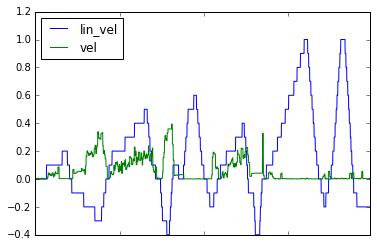
\includegraphics{motion_vs_cmd}
\centering
\caption{Commanded velocity (lin\_vel) as opposed to recorded motion (vel). Vel is always positive because it is measured in terms of euclidian distance moved by the center of the AprilTag between successive updates of the tag tracking. 
Note that while the magnitude of the motion is proportional to the commanded motion, sometimes the robot did not move at all, and when it did move, the recorded velocity is quite noisy. Noise may be removed in software, mechanical failure cannot.} 
\label{motor-speed-fig}
\end{figure}


This approach results in learning bad controls if the system observes the robot during a temporary failure. 
In a system with minimal failures, this problem can be minimized, but as discussed earlier, inexpensive children's toys are not such a system. 

GRITSBots has a calibration step, but the calibration is automated, and is only performed once for each robot, after which it is assumed that the calibration variables are constant.
Calibration can be automated in a homogenous platform with reasonably reliable hardware. 
Non-homogenous platforms require different calibration for different platforms, which reduces the benefit of automation. 
Further, it works against transitioning to a new platform by adding an additional hurdle in the form of developing a new calibration method for the new platform. 

The lack of an automated calibration and control method drove the TinyRobo swarm to use more differential drive vehicles, as they struck a balance between the fully holonomic drive used in the SpiderBots, which is expensive but easy to control, and the Ackerman drive used in inexpensive RC cars, which is less expensive, but has more complex control math \citep{lairdspider}.
It also increases the difficulty of using a heterogenous system, and so operates against the advantages of heterogeneity as discussed in section \todo{automate labeling sections}

\subsection{April Tag Latency}

April tags have very solid position and orientation tracking, but are computationally intensive to detect and localize in typical webcam images. 
More tags leads to longer computation time, increasing the latency of the robot control loop. 
Parallelizing the implementation of the AprilTag library could improve it significantly, but is out of scope for this work. 

One version of the GRITSBots used AprilTags and a standard web cam, resulting in position updates at approximately 10Hz. 
This update rate is consistent with that observed by the author using the ROS implementation of AprilTags. 
Decreasing the size of the image in which the tags are detected speeds it up, at the cost of requiring larger tags in order to have them legible in the lower-resolution image. 
The update rate places an upper bound on the ability of the system to respond to the motion of the robots. 
To decrease the latency of this sensing, the GRITSBots team considered moving to color blob tags, which can be detected by the onboard vision processor of a Pixy CMUCam5 at up to 50Hz \citep{PickemGrits2014}. 

\section{Conclusion}

The origin of the TinyRobo hardware platform was a hobbyist project, intended to combine the diminishing cost and increasing power of Internet of Things (IoT) networking modules with the ready availability of toys to create a system that lowers the barrier to development of multi-robot systems.
While it did not fully achieve this goal, there are a number of lessons that will be relevant to future developers of multi-robot research platforms. 

The drivetrain of the system is of paramount importance. 
Sensors and networking can be virtualized, as in TinyRobo and GRITSBots, but no amount of clever programming will compensate for balky motion. 
The use direct drive, as in GRITSBots or mROBerTO, is encouraged because the resulting drive train will be sealed against foreign matter. 
Further, the use of stepper motors in GRITSBots provides some degree of precision in motion control by directing the motor in steps of known resolution, rather than commanding a particular speed. 
If the system requires additional torque, use sealed micro gearmotors rather than adopting a drivetrain from a toy. 
Toy drivetrains are designed for minimal cost over reliability and precision. 

The chassis of the robot can be constructed from the same printed circuit board (PCB) that the electronics are supported on. 
Over the scales of forces present in tabletop swarms, PCB can be considered completely rigid, and electronics solder provides sufficient mechanical strength for motor mounts. 
The use of custom mechanical assemblies in e.g. Jasmine micro robots adds complexity to the build process. 
Where possible, design to use the PCB instead. 
Using children's toys in TinyRobo was intended to avoid the use of such custom parts, but brought with it additional problems that were outside of the scope of the work to solve, and could have been avoided with a simpler drivetrain. 

Minimize parts count. 
TinyRobo was developed around the ESP-8266 WiFi module because the module includes both a powerful microprocessor and wireless communication. 
Multi-use devices like the ESP-8266 are becoming cheaper and more competent quickly.
The processor in mROBerTO is both a 32-bit ARM processor, a low-power Bluetooth transceiver, and an ANT Wireless tranceiver. 
The VL6180X IC combines an ambient light sensor and a laser-based time-of-flight range sensor in a package measuring approximately 5x8x1mm. 
Reducing parts count reduces cost and speeds assembly. 

Use autonomous charging, and have each robot be able to monitor its own battery level. 
Any operation that requires user intervention with each individual robot will not scale well as the swarm size increases. 
In the case of the Kilobots, the swarm as a whole can be charged in parallel, rather than requiring the individual robots to be connected with a charger. 
For the GRITSBbots, pins on the front of each robot allows the robot to connect to a charging station by itself, rather than requiring a human to connect it. 
The TinyRobo platform could be trivially altered to provide GRITSBots-style self-charging, but does not at present have a method to detect a low battery condition, aside from monitoring the motor drivers for an undervoltage signal. 
The alternative to this, leaving out self-charging and battery monitoring, results in increased effort by humans to keep the batteries charged and failures due to discharged batteries that are not immediately obvious to the control software. 
At a more general level, hardware health monitoring is required for systems that intend to detect their own failed components and work around them, which increases robustness in a swarm system. 
